% Definição do tamanho da letra, folha e estilo.
\documentclass[12pt, a4paper]{article}

% Definição de pacotes.
%% Padrão UTF-8.
%% Texto brasileiro.
%% Identação dos parágrafos.
%% Adição de imagens.
%% Geometria da página de acordo com a ABNT.
\usepackage[utf8]{inputenc}
\usepackage[brazil]{babel}
\usepackage{indentfirst}
\usepackage{graphicx}
\usepackage{float}
\usepackage{geometry}
\geometry{a4paper, left = 3cm, right = 3cm, top = 3cm, bottom = 3cm}

% Numeração da página.
\pagenumbering{arabic}

% Path das imagens.
\graphicspath{{./img/}}

\title{\textbf{Biblioteca LPM - Memória RAM}}
\author{
	Guimarães, João Guilherme M.\\
	\texttt{joaog95@live.com}
}
\date{\today}

\begin{document}
	% Escrever o título, autor e data.
	\maketitle
	
	% Espaçamento vertical
	\vspace{1cm}
	
	\section{Introdução}
	
	\par A biblioteca LPM é uma padronização da indústria para fornecer módulos eficientes e de grande abstração para os projetistas de hardware, e devido sua integração com o Quartus, iremos utilizar o módulo de memória RAM com a configuração de 32 posições por 8 bits.
	
	\section{Objetivos}
	
	\par Com esta prática, espera-se um melhor entendimento do módulo de memória da biblioteca LPM e uma boa assimilação do conteúdo visto em sala de aula sobre o processo de escrita e leitura de dados.
	
	\section{Material}
	
	\par Para realização desta prática, foi utilizado os seguintes equipamentos e softwares:
	
	\begin{itemize}
		\item Logisim 2.7.1;
		\item ModelSim 10.1d;
		\item Quartus 13.0sp1;
		\item FPGA EP2C35F672C6 e
		\item Kernel Linux / SO Deepin 15.11.
	\end{itemize}
	
	\vspace{\baselineskip}	
	

    \section{Desenvolvimento}
    
    \par A primeira aula prática da disciplina de Laboratório de Arquitetura de Computadores II, é dividida em 2 partes, a primeira consiste em simular o módulo de memória RAM da biblioteca LPM e realizar os processos de escrita e leitura. Já a segunda parte, foca em inicializar a memória utilizando um arquivo MIF (\textit{Memory Inicialization File}).
    
    \vspace{\baselineskip}

	\par De acordo com o roteiro de aula, os dados obtidos nas duas práticas deveram ser apresentados em um display de 7-segmentos, sendo assim, foi desenvolvido um módulo decodificador BCD com o auxílio do software Logisim, para criação da Tabela Verdade e para a simplificação das equações.
	
	\vspace{\baselineskip}
    
    \begin{figure}[H]
    	\centering
    	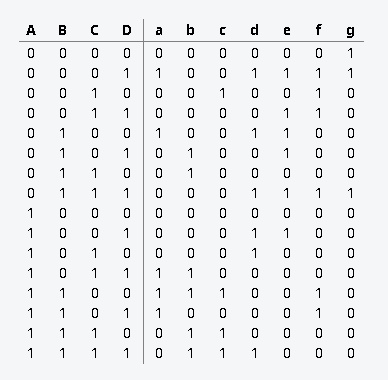
\includegraphics{./TabelaVerdade}
    	\caption{Tabela Verdade para o decodificador BCD}
    	\label{fig: tabela verdade}
    \end{figure}
    
    \par \textit{Obs.: os displays de 7-segmentos da FPGA EP2C35F672C6, possuem a configuração de ânodo comum, sendo assim, para acender os LEDs é necessário a aplicação do sinal 0, e para apagá-los, o sinal 1.}

    \vspace{\baselineskip}
    
    \par A partir da Tabela Verdade apresentada acima, foi obtida as seguintes equações para cada segmento do display:
    
    \begin{figure}[H]
    	\centering
    	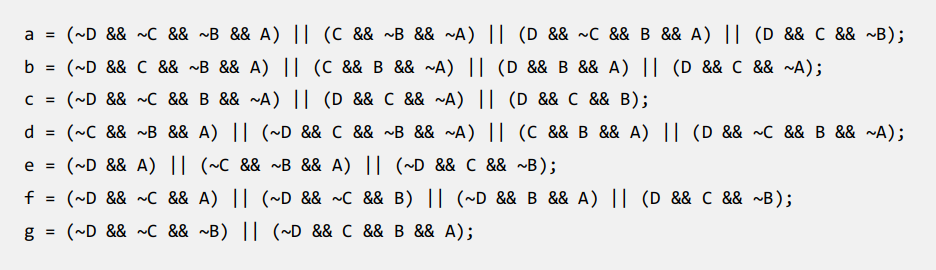
\includegraphics[width=15cm]{./equacoes}
    	\caption{Equações simplificadas para cada segmento do display}
    	\label{fig: equacoes}
    \end{figure}

    \vspace{\baselineskip}
    
    \par Com o módulo decodificador finalizado, foi dado prosseguimento a criação da memória RAM utilizando a biblioteca LPM e seu respectivo arquivo de inicialização. Para tal, foi seguido o tutorial fornecido em sala e obtivemos o seguinte resultado:
    
    \vspace{\baselineskip}
    
    \begin{figure}[H]
    	\centering
    	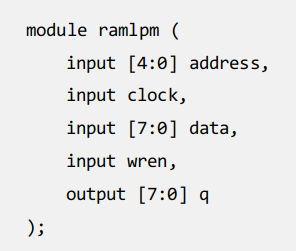
\includegraphics[width=5cm]{./ramlpm}
    	\caption{Assinatura do módulo da memória RAM}
    	\label{fig: ramlpm}
    \end{figure}

	\begin{figure}[H]
		\centering
		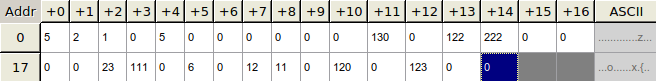
\includegraphics[width=15cm]{./mif}
		\caption{Exibição do arquivo MIF}
		\label{fig: mif}
	\end{figure}

	\section{Simulação}
	
	\subsection{Parte I}
	
	\par Para simplificar o processo de simulação, o módulo de memória e decodificador foram testados separadamente, e seguem abaixo:
	
	\begin{figure}[H]
		\centering
		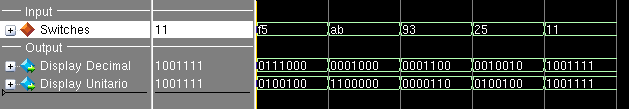
\includegraphics[width=15cm]{./decoder}
		\caption{Simulação do Decodificador BCD}
		\label{fig: decoder}
	\end{figure}

	\begin{figure}[H]
		\centering
		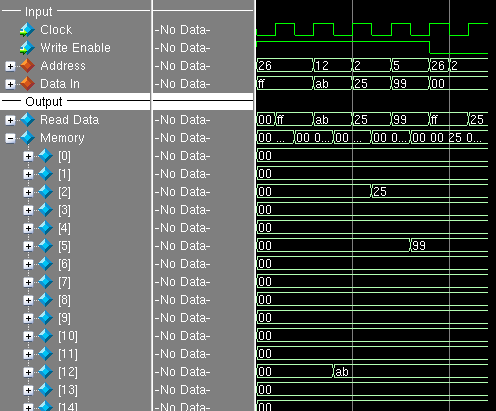
\includegraphics[width=13cm]{./memory}
		\caption{Simulação da Memória}
		\label{fig: memory}
	\end{figure}

	\par Analisando a figura \ref{fig: memory}, é possível perceber que a implementação da memória RAM pela biblioteca LPM, realiza o processo de leitura na borda de subida do \textit{Clock}, e a escrita na borda de descida. Esta implementação se assemelha com que acontece normalmente em processadores que aproveitam do Pipeline, como foi visto na disciplina de Arquitetura de Computadores I.
	
	\subsection{Parte II}
	
	\par Como dito anteriormente, a prática II consiste na inicialização da memória utilizando o arquivo MIF apresentado na figura \ref{fig: mif}.
	
	\begin{figure}[H]
		\centering
		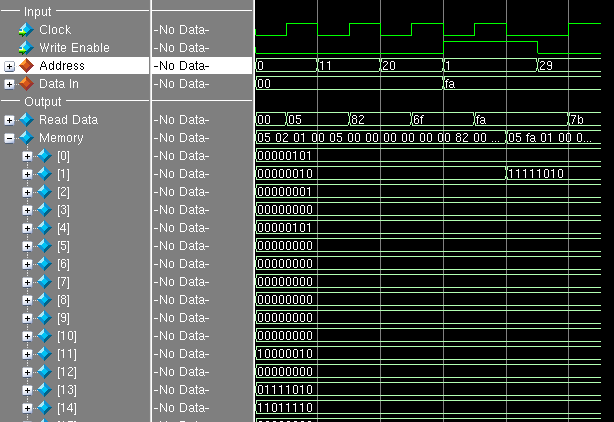
\includegraphics[width=15cm]{./memory_mif}
		\caption{Simulação da Memória inicializada com o MIF}
		\label{fig: memory and mif}
	\end{figure}

	\par A simulação da figura \ref{fig: memory and mif}, foi feita realizando a leitura das posições 11, 20 e 29, e a escrita na posição 1 no terceiro ciclo do \textit{Clock}.
	
	\vspace{\baselineskip}
	
	\par \textit{Obs.: como o módulo decodificador foi reaproveitado, sua respectiva simulação não foi refeita.}
    

	\section{Conclusão}
	
	\par Com a execução desta prática, pudemos aperfeiçoar nossos conhecimentos nas bibliotecas do Quartus, na linguagem Verilog, além de assimilar melhor o conteúdo dado em sala de aula.

\end{document}
	